% **************************************************
% Macro specifiche per il documento corrente
% **************************************************
% Nome
\newcommand{\docName}{Specifica tecnica}
% Nome file
\newcommand{\docFileName}{specifica\_tecnica.1.0.pdf}
% Versione
\newcommand{\docVers}{0.1}
% Data creazione
\newcommand{\creationDate}{2013-01-16}
% Data ultima modifica
\newcommand{\modificationDate}{2013-01-17}
% Stato in {Approvato, Non approvato}
\newcommand{\docState}{Non approvato}
% Uso in {Interno, Esterno}
\newcommand{\docUsage}{Interno}
% Destinatari da specificare come nome1\\ &nome2\\ ecc.
\newcommand{\docDistributionList}{Team SoftwareSynthesis}
% Redattori da specificare come nome1\\ &nome2\\ ecc.
\newcommand{\docAuthors}{}
% Approvato da
\newcommand{\approvedBy}{}
% Verificatori
\newcommand{\verifiedBy}{}
% Perscorso (relativo o assoluto) che punta alla directory contenente shared/
% come sua sottodirectory (per comodità chiamiamola 'doc root').
\newcommand{\docRoot}{..}
% definire se si vuole l'indice delle tabelle
\def\INDICETABELLE{false}
% definire se si vuole l'indice delle figure
\def\INDICEFIGURE{false}

% importa il preambolo condiviso da tutti i documenti
% shared/preamble.tex
%
% Questo documento contiene la parte del preambolo condivisa e viene pertanto
% richiamato nel 'master' di tutti i documenti di progetto.  Al suo interno
% contiene le inclusioni (e le configurazioni) di tutti i package richiesti per
% la compilazione dei documenti, le macro di carattere generale e la definizione
% degli stili di pagina.

\documentclass[a4paper,10pt,openright]{article}

% **************************************************
% Macro generiche
% **************************************************
\newcommand{\team}{Software Synthesis}                    % chi siamo
\newcommand{\email}{software.synthesis@gmail.com}         % e-mail
\newcommand{\caName}{}                                    % titolo capitolato
\newcommand{\caDescr}{}                                   % descrizione
\newcommand{\inglese}[1]{\textit{#1}}

% **************************************************
% Codifica e lingua dei documenti
% **************************************************
\usepackage[utf8x]{inputenc}                              % codifica caratteri dei documenti sorgenti
\usepackage[english,italian]{babel}                       % localizzazione ai fini di sillabazione e cross-references
\usepackage[T1]{fontenc}                                  % codifica font di output

% **************************************************
% Definizione geometria della pagina
% **************************************************
\usepackage[a4paper,head=4cm,top=4.5cm,bottom=3cm,left=3cm,right=3cm,bindingoffset=5mm]{geometry}

% *************************************************
% Intestazioni e piè di pagina personalizzati
% *************************************************
\usepackage{fancyhdr}
% stile normale
\fancypagestyle{normal}{
\fancyhead{}                                              % intestazione
\fancyhead[RE,RO]{
\begin{picture}(0,0)
  \put(-410,0){
\includegraphics[width=1.02\textwidth]{header_logo}}
  \put(-410,10){\sffamily\large\leftmark}
\end{picture}
\vspace{-4pt}
}
\renewcommand{\headrulewidth}{.4pt}                       % riga sotto l'intestazione
\cfoot{}                                                  % piè di pagina
\fancyfoot[RO,LE]{\sffamily
  pag.~\thepage{} di \pageref{LastPage}}                  % a dx nelle pag. dispari e a sx in quelle pari
\fancyfoot[RE,LO]{\sffamily\docFileName{} -- v.\docVers}
\renewcommand{\footrulewidth}{.4pt}                       % riga sopra il piè di pagina
}
% stile per gli indici
\fancypagestyle{toc}{
\fancyhead{}                                              % intestazione
\fancyhead[RE,RO]{
\begin{picture}(0,0)
  \put(-410,0){
\includegraphics[width=1.02\textwidth]{header_logo}}
\end{picture}
}
\renewcommand{\headrule}{}                                % nessuna riga sotto l'intestazione
\cfoot{}                                                  % piè di pagina
\fancyfoot[RO,LE]{\sffamily\thepage{}}                    % a dx nelle pag. dispari e a sx in quelle pari
\fancyfoot[RE,LO]{\sffamily\docFileName{} -- v.\docVers}
\renewcommand{\footrulewidth}{.4pt}                       % riga sopra il piè di pagina
}

\pagestyle{fancy}                                         % premetto: non so usare bene le marche:
\renewcommand{\sectionmark}[1]{\markboth{#1}{#1}}         % se qualcuno ha idee migliori si faccia avanti!

% **************************************************
% Tabelle
% **************************************************
\usepackage{tabularx}                                     % tabelle di larghezza fissa con una o più colonne variabili
\usepackage{multirow}                                     % colonne con colonne che si estendono per più righe
\usepackage{booktabs}                                     % per inserire l'ambiente table e le righe orizz. nelle tabelle
\usepackage{longtable}			                          % tabelle oltre i limiti di pagina

% **************************************************
% Cross-references e collegamenti ipertestuali
% **************************************************
\usepackage[hidelinks]{hyperref}
\hypersetup{%
  colorlinks=false, linktocpage=false, pdfborder={0,0,0}, pdfstartpage=3, pdfstartview=FitV,%
  urlcolor=Cyan, linkcolor=Cyan, citecolor=Black, %pagecolor=Black,%
  pdftitle={\docName}, pdfauthor={\team}, pdfsubject={}, pdfkeywords={},%
  pdfcreator={pdflatex}, pdfproducer={pdflatex with hyperref package}%
}

% **************************************************
% Immagini e grafica
% **************************************************
\usepackage{graphicx}                                     % supporto ad aspetti avanzati delle immagini
\graphicspath{{\docRoot/pics/}}                           % percorso contenente tutti i file immagini
\usepackage{color}                                        % permette di colorare facilmente il testo

% **************************************************
% Altri pacchetti opzionali
% **************************************************     
\usepackage{lastpage}                                     % per sapere il numero totale di pagine
\usepackage{lipsum}                                       % genera "dummy text" per prove di impaginazione
\usepackage{eurosym}                                      % per il simbolo dell'euro usare \EUR{x} dove x è l'importo


% Fine del preambolo e inizio del documento
\begin{document}

% Inclusione della prima pagina
% shared/firstpage.tex
%
% Questo documento definisce il contenuto della prima pagina, che si suppone
% essere uguale in tutti i documenti.  Oltre al logo e al titolo, la prima
% pagina contiene i metadati relativi al documento in cui viene inclusa.


% rimuove intestazioni e piè di pagina
\pagestyle{empty}

\begin{center}

% logo del gruppo

\includegraphics[width=1.5\textwidth]{logo}

\vspace{1in}

% titolo del documento
{\Huge\bfseries \docName}

\vspace{1in}

% tabella riepilogativa
\begin{tabularx}{.7\textwidth}{>{\bfseries\sffamily}l>{\sffamily}l}
\toprule
\multicolumn{2}{>{\sffamily}c}{Informazioni sul documento}\\
\midrule
Nome file:            & \docFileName\\
Versione:             & \docVers\\
Data creazione:       & \creationDate\\
Data ultima modifica: & \modificationDate\\
Stato:                & \docState\\
Uso:                  & \docUsage\\
Redattori:            & \docAuthors\\
Approvato da:         & \approvedBy\\
Verificatori:         & \verifiedBy\\
\bottomrule
\end{tabularx}

\end{center}

\newpage


%---------------------------RUOLI----------------------------
%FASE 1:
%Progettisti: TRES, STEFANO, SCHIVO;
%FASE 2:
%Progettisti: DIEGO, ELENA, RIZZI

%Verificatore: Andrea Meneghinello
%Responsabile finale TRES
%------------------------------------------------------------

% Storico delle modifiche
\section*{Storia delle modifiche}
\begin{center}
\begin{longtable}{lp{.32\textwidth}lll}
\toprule
Versione & Descrizione intervento & Membro & Ruolo & Data\\
\midrule % inserire qui il contenuto della tabella
0.2 & Stesura dell'introduzione ai design pattern. Stesura dell'introduzione ai tracciamenti. & Stefano Farronato & Progettista & 2013-01-17\\
0.1 & Creazione del documento e stesura della sezione ``Introduzione''. & Riccardo Tresoldi & Progettista & 2013-01-16\\
\bottomrule
\end{longtable}
\end{center}
\newpage

% inclusione dell'indice
% shared/toc.tex
%
% Questo file contiene le istruzioni che generano l'indice o gli indici del
% documento (utile nel caso in cui decidessimo di avere anche un indice delle
% tabelle e/o un indice delle figure).

\pagestyle{toc}
\pagenumbering{roman}

\tableofcontents

\newpage


% Alcuni aggiustamenti per le pagine
\pagenumbering{arabic}
\setcounter{page}{1}
\pagestyle{normal}

% Qui ha inizio il documento vero e proprio...

\newpage

\section{Introduzione}
\subsection{Scopo del prodotto}
\purpose

\subsection{Scopo del documento}
Il presente documento è stato redatto al fine di produrre le specifiche sulla progettazione ad alto livello, del prodotto MyTalk. A tal fine il documento presenterà:

\begin{itemize}
	\item Un elenco con le specifiche dei design pattern utilizzati.
	\item Una descrizione dettagliata dei componenti rilevati in fase di progettazione indicando il tipo,
la funzione e l'obbiettivo.
	\item L'architettura d'alto livello del sistema.
	\item I diagrammi UML per definire i flussi principali di controllo dell'applicativo.
	\item Il tracciamento dei requisiti e delle componenti, negli schemi: requisiti-componenti e componenti-requisiti.
\end{itemize}

\subsection{Glossario}
\glossaryIntro

\clearpage
\section{Riferimenti}

\subsection{Normativi}
\begin{itemize}
\item[] \textit{piano\_di\_qualifica.2.0.pdf} allegato.
\item[] \textit{norme\_di\_progetto.2.0.pdf} allegato.
\item[] \textit{analisi\_dei\_requisiti.2.0.pdf} allegato
\end{itemize}

\subsection{Informativi}
\begin{itemize}
\item[] Capitolato d'appalto: \caName{}, v1.0, redatto e rilasciato dal proponente Zucchetti s.r.l. reperibile all'indirizzo \url{http://www.math.unipd.it/~tullio/IS-1/2012/Progetto/C1.pdf};
\item[] testo di consultazione: \textit{Software Engineering (8th edition) Ian Sommerville, Pearson Education | Addison Wesley};
\item[] manuale all'utilizzo dei design pattens: \textit{Design Patterns, Elementi per il riuso di software a oggetti - (1/Ed. italiana) Eric Gamma, Richard Helm, Ralph Johnson, John Vlissides, Pearson Education};
\item[] \textit{glossario.1.0.pdf} allegato.
\end{itemize}

\section{Strumenti utilizzati}
\subsection{Java}

\subsection{Hibernate}

%TODO: da completare

\clearpage
\section{Design Pattern}
In questa sezione discuteremo i design pattern utilizzati nella progettazione delle componenti. Ogni design pattern sarà proposto con la seguente forma:

\begin{itemize}
	\item \textbf{Scopo}: verrà proposto lo scopo generico del pattern, al fine di evidenziare subito la sua utilità.
	\item \textbf{Diagramma esemplificativo}: si riporterà lo schema UML, rappresentante un implementazione generica del design pattern in esame.
	\item \textbf{Vantaggi derivanti}: si darà un elenco dei vantaggi apportati dall'utilizzo del pattern, in particolare sotto il profilo della manutenzione e del riuso del codice.
	\item \textbf{Componenti che lo implementano}: infine verranno elencati i componenti dell'architettura di sistema, che implementano il pattern descritto.
\end{itemize}

Per una visione d'insieme dei delle componenti utilizzate da un pattern, e dei pattern utilizzati da un componente, rimandiamo alle sottosezioni ``Tracciamenti Componenti-Design Pattern'' e ``Tracciamenti Design Pattern-Componenti'' della sezione ``Tracciamenti''.


%\subsection{Adapter}
%\subsubsection{Scopo}
%Convertire l'interfaccia di una classe in un altra interfaccia richiesta dal \underline{client} e consente a classi diverse di operare insieme quando ciò non sarebbe altrimenti possibile a causa di interfacce incompatibili.
%\subsubsection{Diagramma esemplificativo}
%\begin{figure}[h]
%\centering
%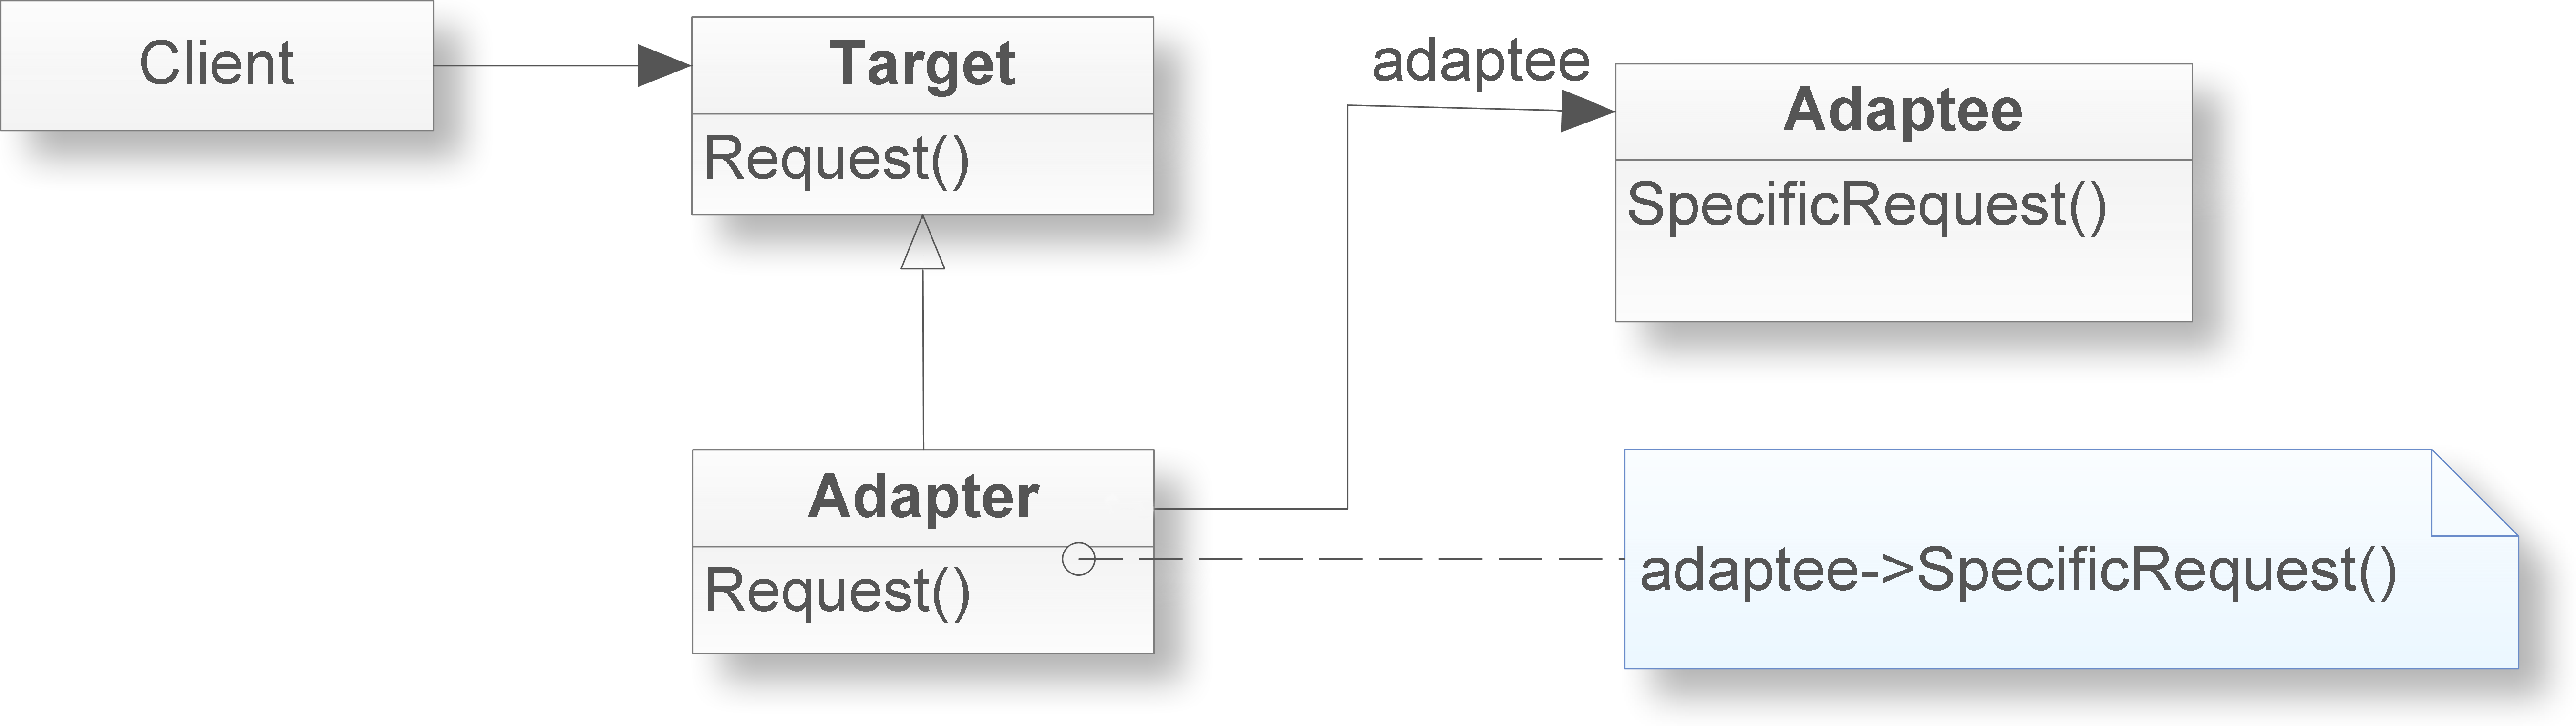
\includegraphics[width=.8\textwidth]{adapter}
%\caption{Diagramma ad alto livello del pattern Adapter.}\label{fig:adapter}
%\end{figure}
%\subsubsection{Vantaggi derivanti}
%\begin{itemize}
%\item consente di adattare una classe esistente senza doverla ridefinire;
%\item un unico oggetto può adattare più classi.
%\end{itemize}
%\subsubsection{Componenti che lo implementano}

\subsection{Composite}
\subsubsection{Scopo}
Il pattern Composite ha lo scopo di comporre oggetti in strutture ad albero al fine di rappresentare gerarchie parte-tutto e consentire ai \underline{client} di trattare oggetti singoli e composizioni in modo uniforme. Permette inoltre di gestire strutture dati gerarchicizzate con elementi ``foglie'' ed elementi ``contenitori'', l'ideale per la struttura ``gruppo'' e ``utente''.
\subsubsection{Diagramma esemplificativo}
\begin{figure}[h]
\centering
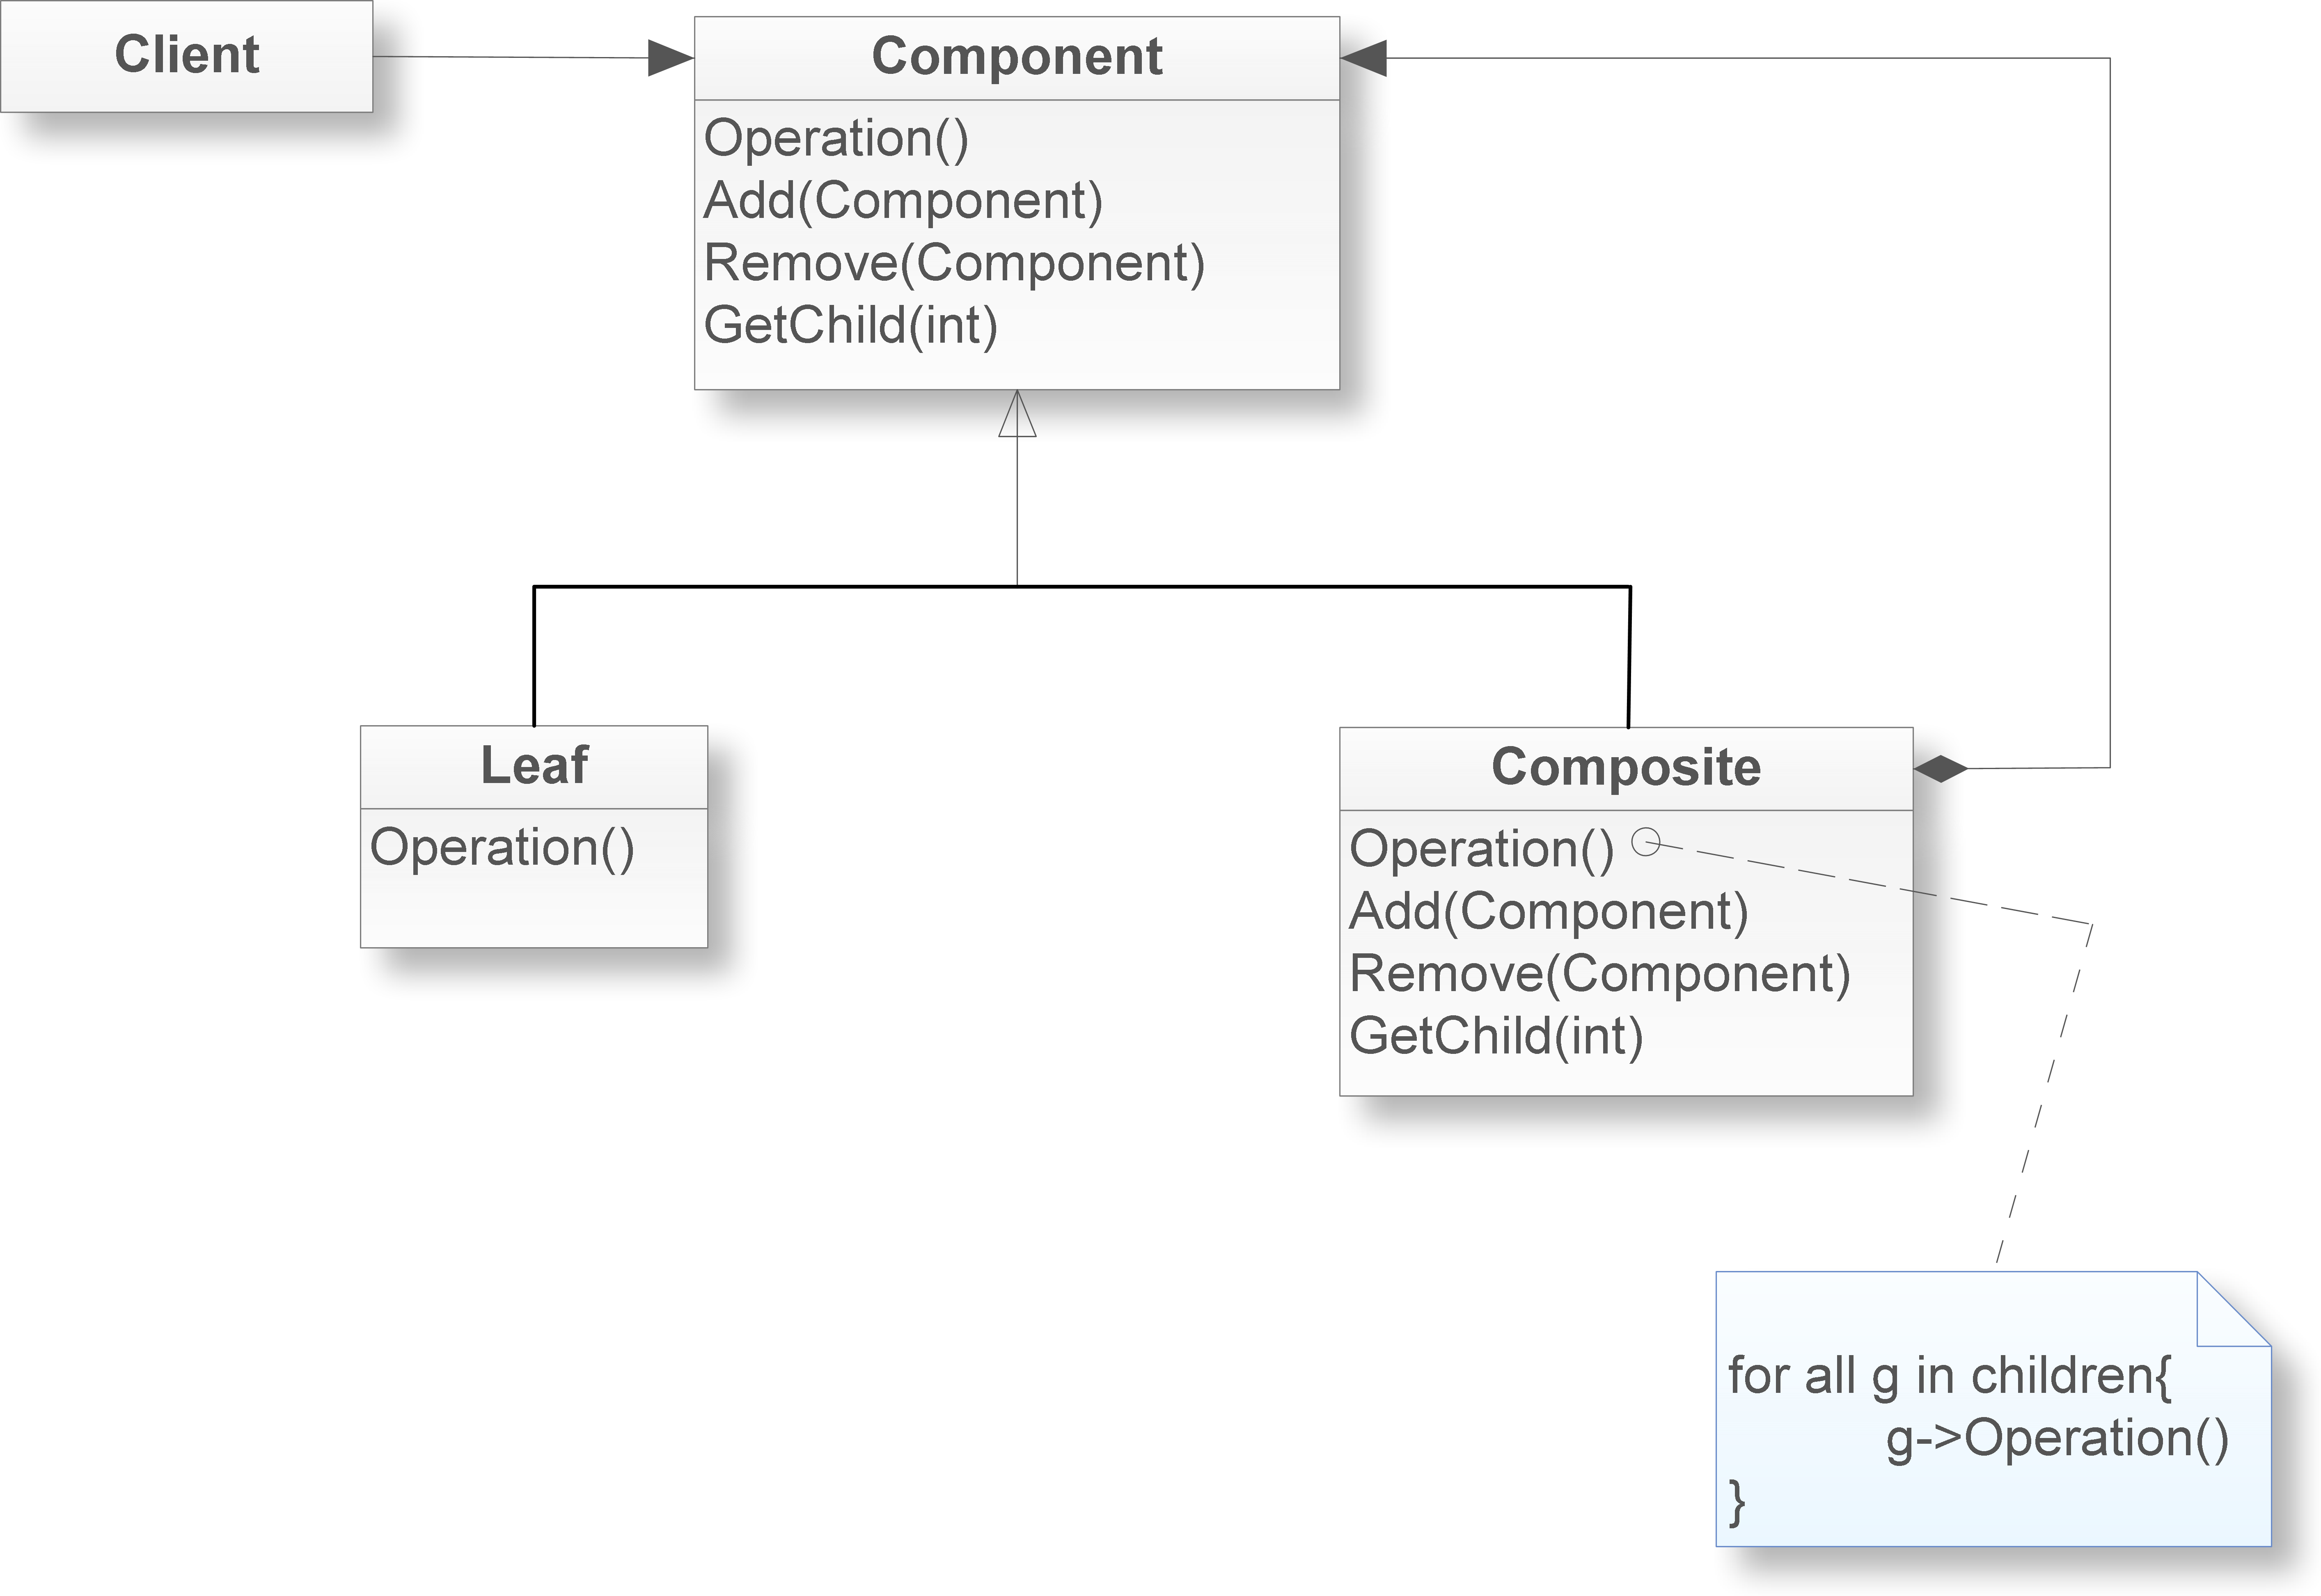
\includegraphics[width=.8\textwidth]{composite}
\caption{Diagramma ad alto livello del pattern Composite.}\label{fig:composite}
\end{figure}
\subsubsection{Componenti che lo implementano}
\begin{description}
\item{\bfseries\scshape Gestione della rubrica (lato server)}\\
Composite permette di trattare in maniera omogenea singoli oggetti e oggetti composti, come gli utenti e gruppi di utenti della rubrica. Inoltre, visto che rende più semplice l'aggiunta di componenti, permetterebbe in futuro l'integrazione di nuove tipologie di utenti senza la necessità di modificare la struttura preesistente.

Lo svantaggio principale che comporta l'uso di Composite è la mancanza di limiti nell'aggiunta di nuove tipologie di componenti. Per far fronte a questo rischio si è introdotta la classe \texttt{org.softwaresynthesis.mytalk.server.abook.AddressBook} che controlla l'accesso alla struttura dati corrispondente alla rubrica.
\end{description}

\subsection{Data Access Object (DAO)}
\subsubsection{Scopo}
Il pattern DAO ha lo scopo di disaccoppiare la logica di business dalla logica di accesso ai dati. Questo si ottiene spostando la logica di accesso ai dati dai componenti di business ad una classe DAO rendendo i componenti che implementano la logica di business indipendenti dalla natura del dispositivo di persistenza. Questo approccio garantisce che un eventuale cambiamento del dispositivo di persistenza non comporti modifiche sui componenti di business.

\subsubsection{Diagramma esemplificativo}
\begin{figure}[h]
\centering
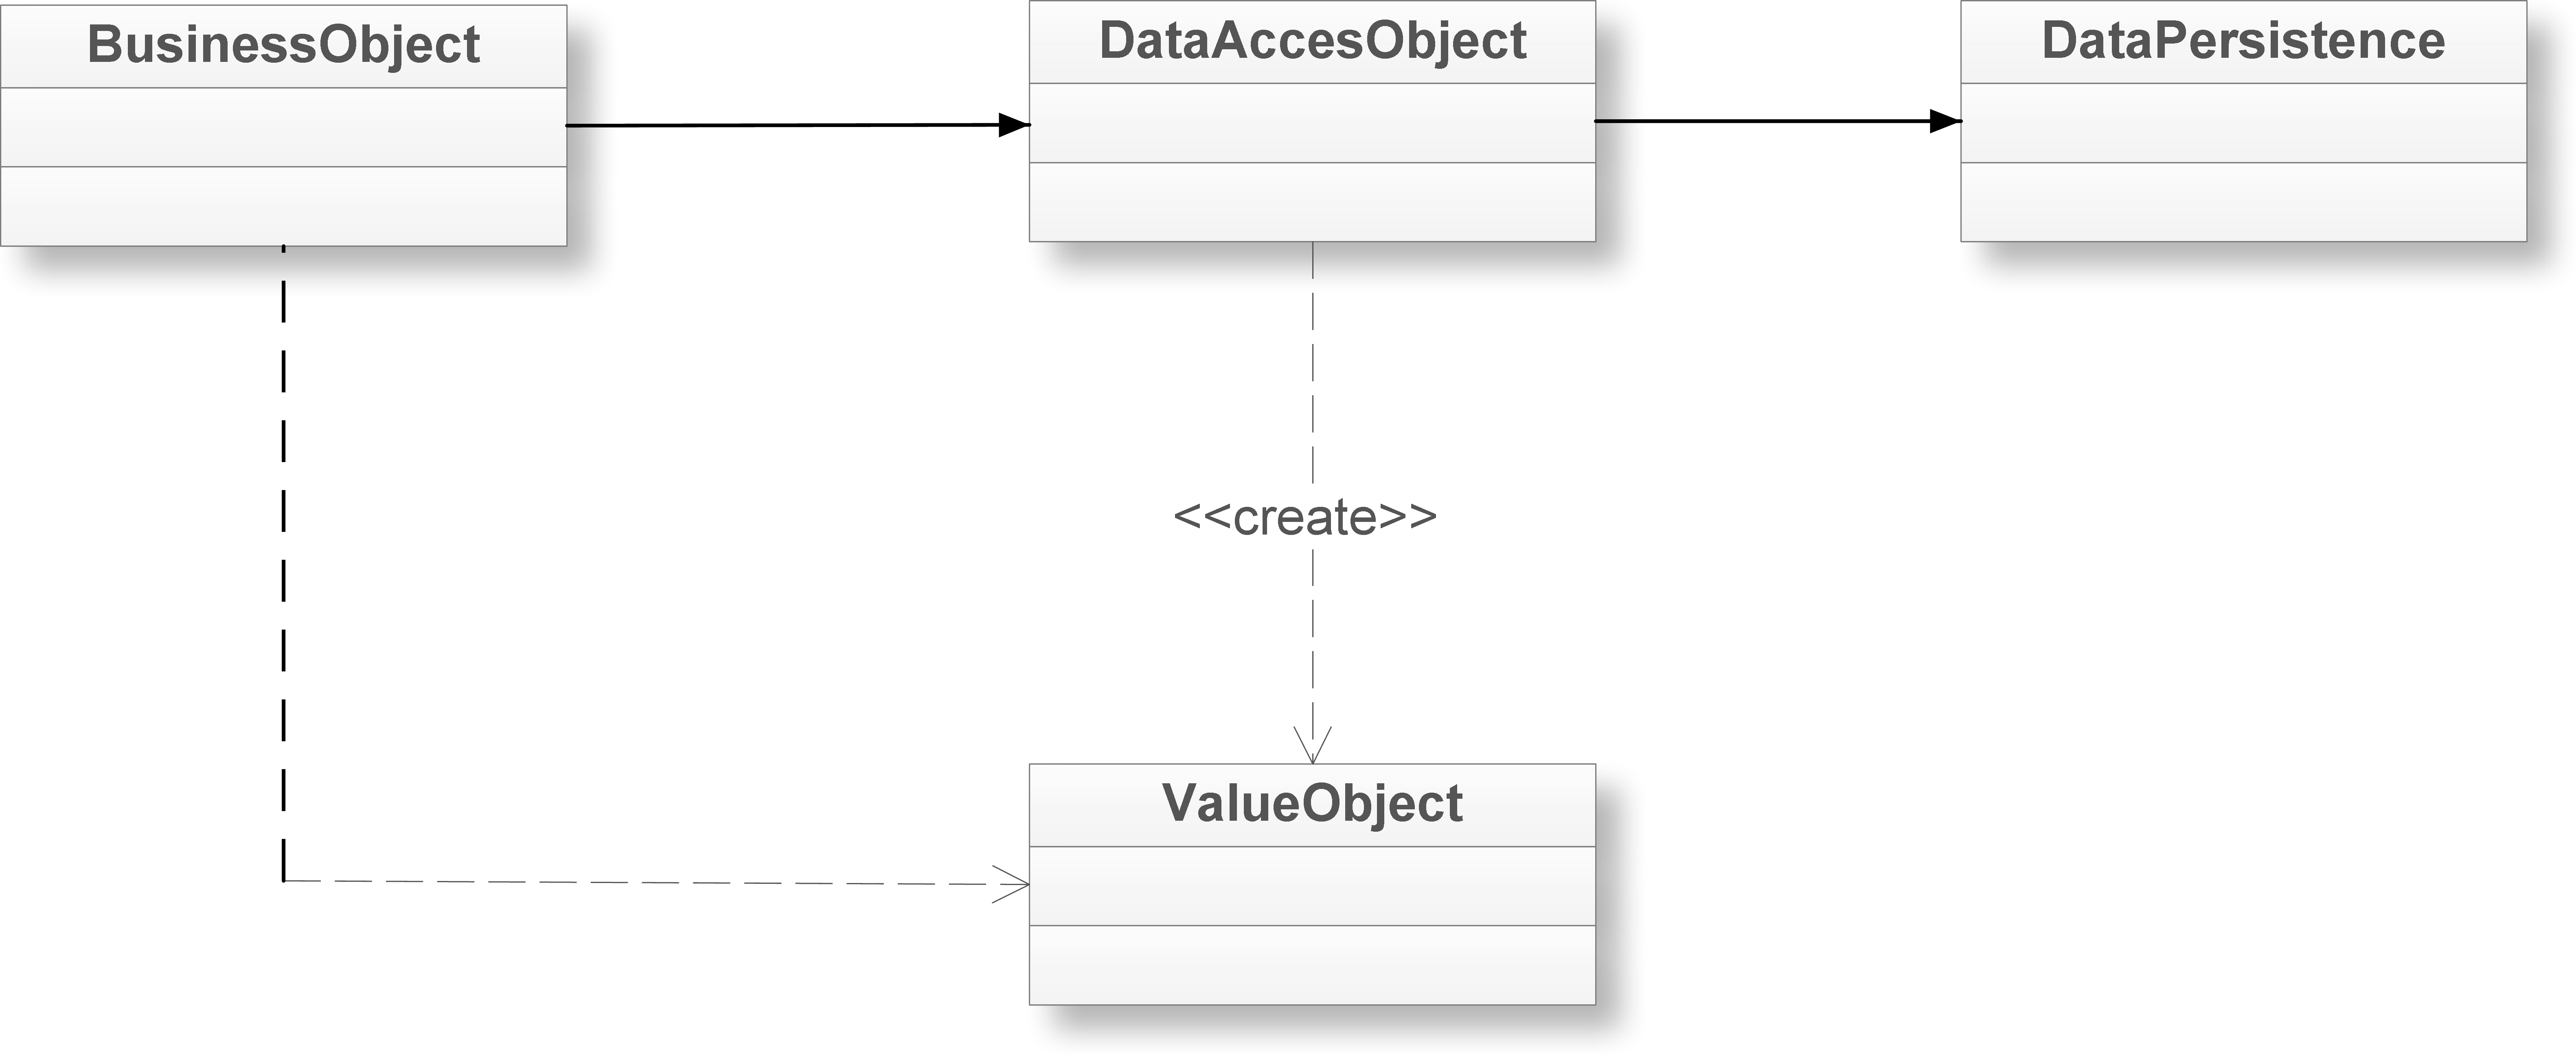
\includegraphics[width=.8\textwidth]{dao}
\caption{Diagramma ad alto livello del pattern DataAccessObject.}\label{fig:dao}
\end{figure}

\subsubsection{Componenti che lo implementano}
\begin{description}
\item{\scshape\bfseries Gestione Database}\\
Le classi DAO consentono di isolare l'accesso alle tabelle del database dalla parte di business logic facendo corrispondere alle invocazioni di metodo le opportune operazioni sui record del database. L'utilizzo di tale pattern crea inoltre un maggiore livello di astrazione e mantiene una rigida separazione tra i sottosistemi corrispondenti a model e presenter.
\end{description}

\subsection{Façade}
\subsubsection{Scopo}
Fornire un interfaccia unificata per un insieme di interfacce presenti in un sottosistema. Façade definisce un interfaccia di livello più alto che rende il sottosistema più semplice da utilizzare.

\subsubsection{Diagramma esemplificativo}
\begin{figure}[h]
\centering
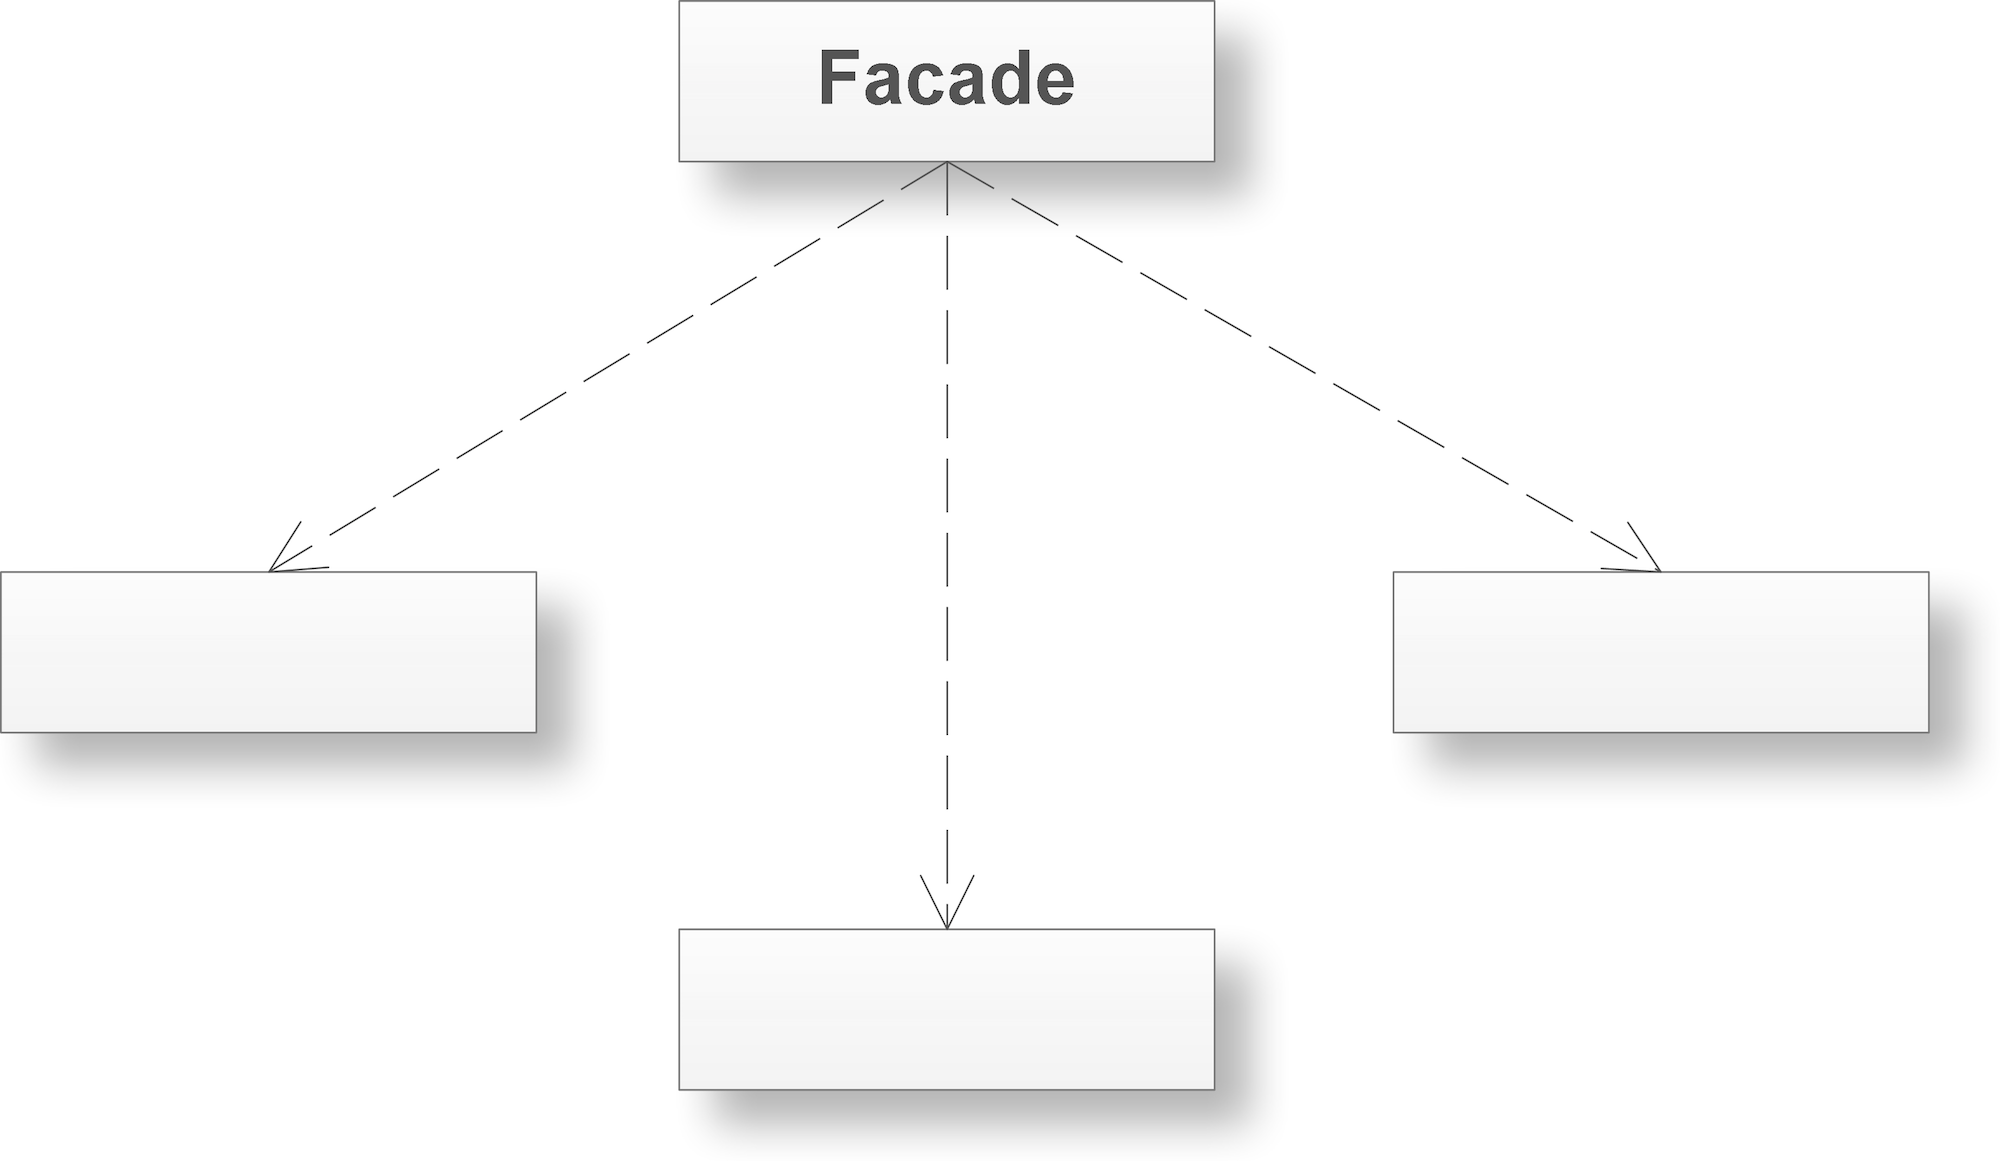
\includegraphics[width=.8\textwidth]{facade}
\caption{Diagramma ad alto livello del pattern Facade.}\label{fig:facade}
\end{figure}

\subsubsection{Componenti che lo implementano}
\begin{description}
  \item{\scshape \bfseries Façade del server}\\
  L'uso di Façade permette di esporre verso i client una sorta di interfaccia semplificata nascondendo i componenti del sottosistema \texttt{server}, fornendo un punto di accesso centralizzato e riducendo il numero di dipendenze funzionali fra le classi del server e i componenti appartenenti a sottosistemi esterni.
  \item{\scshape \bfseries Façade del presenter}\\
Tramite questo design pattern si introduce un livello di indirettezza fra il sottosistema \texttt{clientpresenter} e \texttt{clientview} con il vantaggio di rendere i due sottosistemi indipendenti.
\end{description}

\subsection{Factory Method}
\subsubsection{Scopo}
Definisce un'interfaccia per la creazione di un oggetto, lasciando alle sottoclassi la decisione sulla classe che deve essere istanziata e consente di deferire l'istanziazione di una classe alle sottoclassi.

\subsubsection{Diagramma esemplificativo}
\begin{figure}[h]
\centering
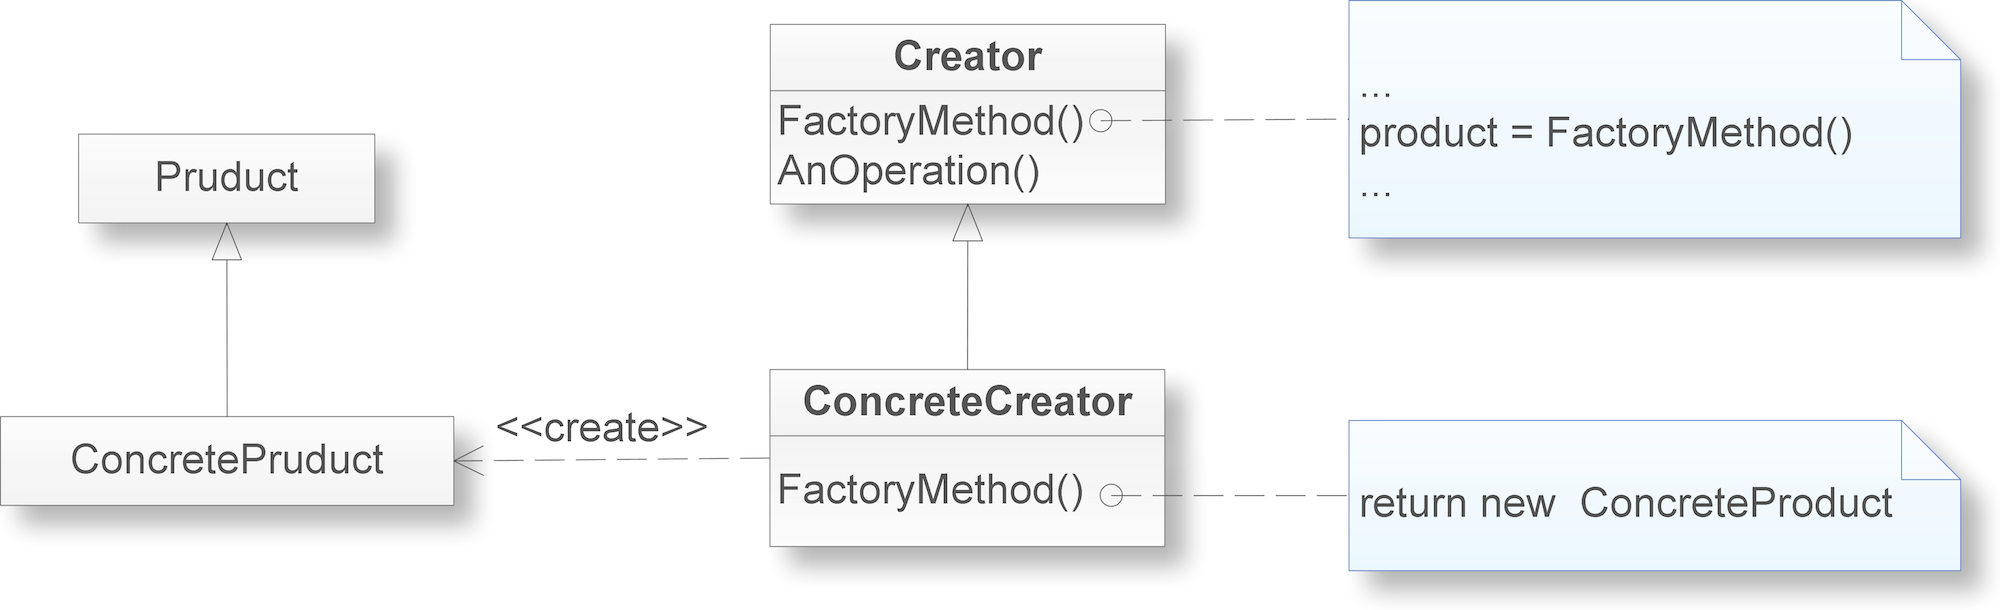
\includegraphics[width=.8\textwidth]{factory_method}
\caption{Diagramma ad alto livello del pattern Factory Method.}\label{fig:factory_method}
\end{figure}

%\subsubsection{Vantaggi derivanti}
%\begin{itemize}
%\item fornisce un punto di aggancio per le sottoclassi per la produzione di una versione specializzata di un oggetto;
%\item connette gerarchie di classi parallele;
%\end{itemize}
\subsubsection{Componenti che lo implementano}
\begin{description}
  \item{\scshape\ttfamily Facade del server}\\
Factory Method permette ai client di ottenere con facilità degli oggetti proxy che specializzano le interfacce \texttt{server.dao.IAudioMessage}, \texttt{server.dao.IAudioVideoMessage} e \texttt{server.dao.IUserData}. Questo permette di ridurre il traffico di rete in quanto oggetti potenzialmente di grandi dimensioni rimangono sul server e vengono scaricati solo quando se ne presenta l'effettiva necessità.
%TODO: Un altro oggetto specializzato che si ottiene mediante il ServerFacade è l'Adapter per la connessione di rete (da definire!)
\end{description}

\subsection{Model-View-Presenter}
\subsubsection{Scopo}
Il pattern architetturale \foreignlanguage{english}{Model-View-Presenter} similmente a quanto accade per \foreignlanguage{english}{Model-View-Controller} (MVC), ha lo scopo di mantenere separata la \textit{business logic}, cioè la gestione dei dati secondo le regole di un determinato dominio e la loro memorizzazione in forma persistente, dalla presentazione e manipolazione mediante interfaccia utente.
\subsubsection{Diagramma esemplificativo}
\begin{figure}[h]
\centering
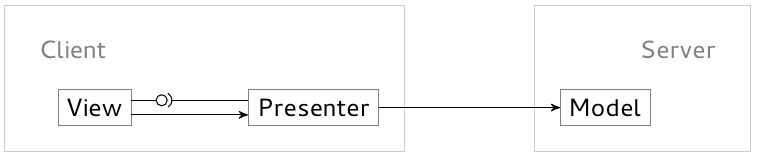
\includegraphics[width=.8\textwidth]{mvpHLdiagram}
\caption{Diagramma ad alto livello del pattern MVP.}\label{fig:mvpHL}
\end{figure}

\subsubsection{Componenti che lo implementano}
MVP viene utilizzato come il pattern più ad alto livello del nostro sistema. La distinzione fra \textit{model}, \textit{presenter} e \textit{view} è infatti rispecchiata dalla suddivisione dell'architettura nei tre sottosistemi \texttt{server}, \texttt{clientpresenter} e \texttt{clientview}.

In generale, l'utilizzo di MVP riduce l'accoppiamento tra i sottosistemi minimizzando le modifiche richieste a ognuno di essi come conseguenza di cambiamenti all'interno degli altri.

Inoltre, le componenti di questo sottosistema non sono vincolate a utilizzare la rete per accedere alle informazioni che sono memorizzate sul server quando queste sono già disponibili (e possono essere elaborate) sul client, migliorando l'esperienza utente.

In particolare, le parti del sistema che utilizzano questo pattern corrispondono ai sottosistemi:
\begin{description}
  \item{\ttfamily server}
  \item{\ttfamily clientpresenter}
  \item{\ttfamily clientview} 
\end{description}

\subsection{Observer}
\subsubsection{Scopo}
Definire una dipendenza uno a molti fra oggetti, in modo tale che se un oggetto cambia il suo stato tutti gli oggetti dipendenti da questo siano notificati e aggiornati automaticamente.
\subsubsection{Diagramma esemplificativo}
\begin{figure}[h]
\centering
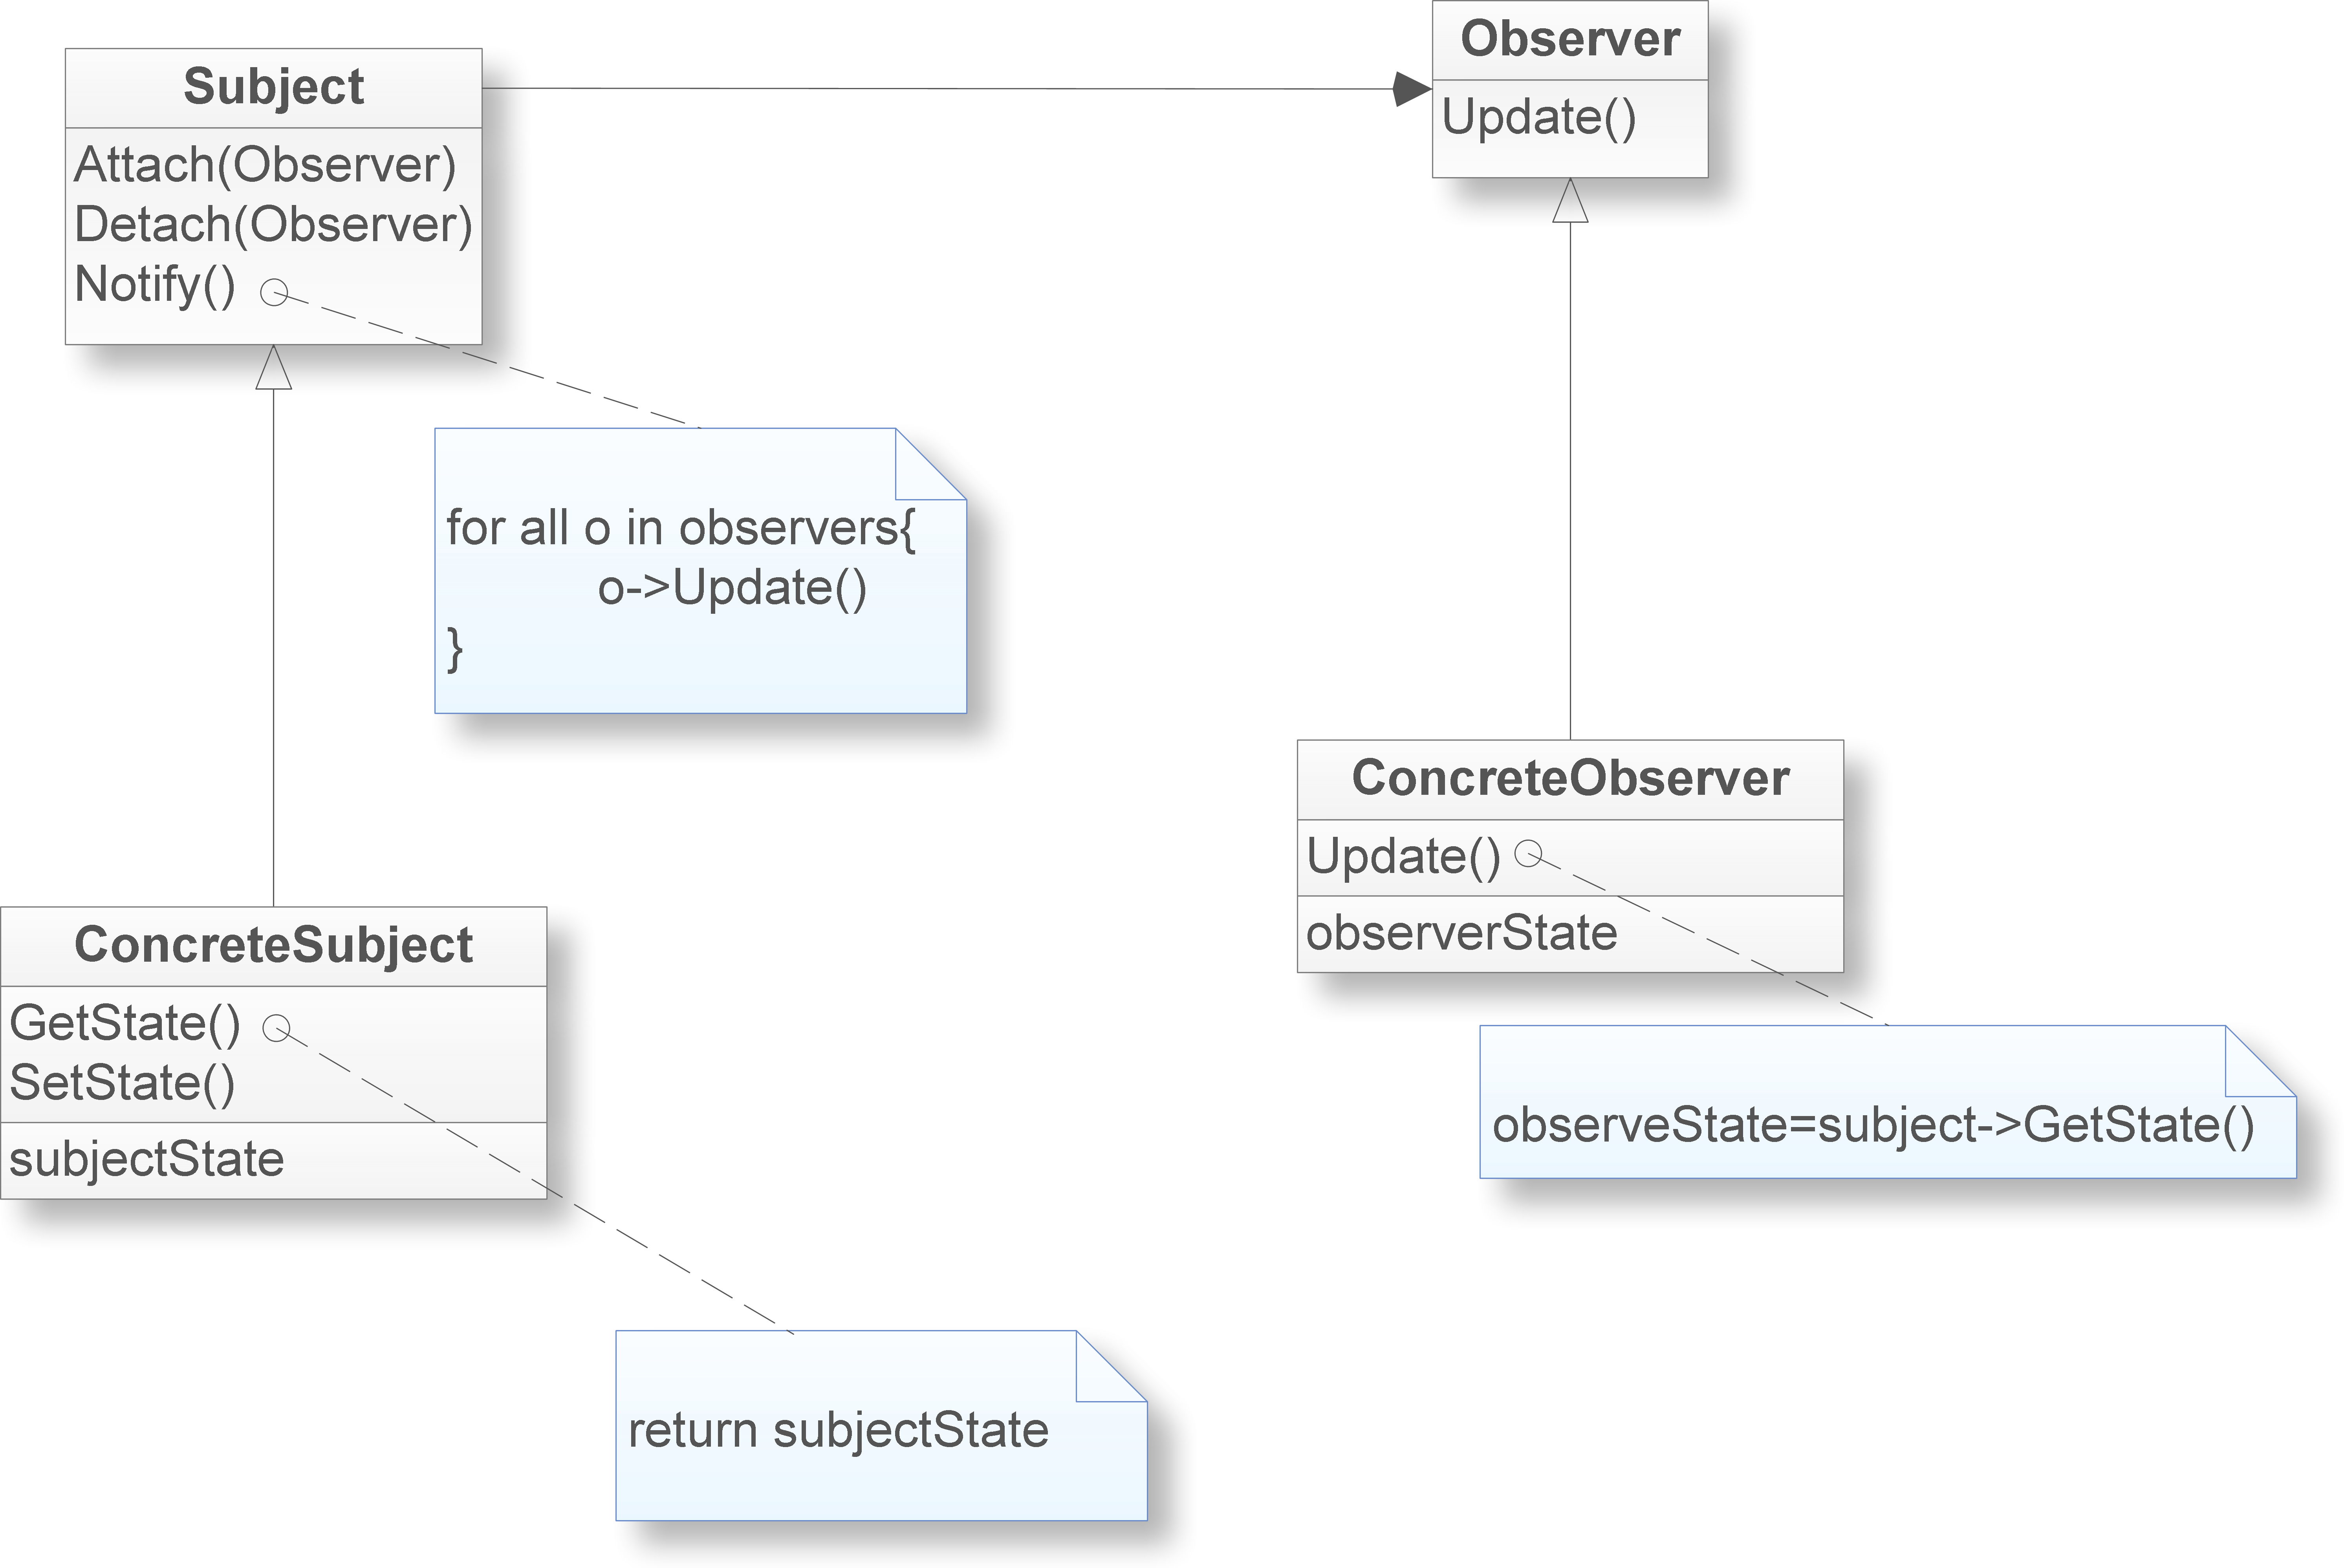
\includegraphics[width=.7\textwidth]{observer}
\caption{Diagramma ad alto livello del pattern Observer.}\label{fig:observer}
\end{figure}
\subsubsection{Vantaggi derivanti}
\begin{itemize}
\item l'oggetto osservato e l'oggetto osservatore non sono legati rigidamente, dunque possono appartenere a livelli di astrazione differenti;
\item l'oggetto osservato notifica automaticamente a tutti gli osservatori
\item 
\end{itemize}
\subsubsection{Componenti che lo implementano}

\subsection{Singleton}
\subsubsection{Scopo}
Il pattern creazionale Singleton, garantisce che una determinata classe possa essere istanziata una sola volta, e di fornirne un punto di accesso globale. Questo pattern va utilizzato negli ambiti in cui si ha la necessità che l'accesso ad una determinata entità sia unico, in modo da permettere la gestione ottimale della risorsa stessa.
\subsubsection{Diagramma esemplificativo}
\begin{figure}[h]
\centering
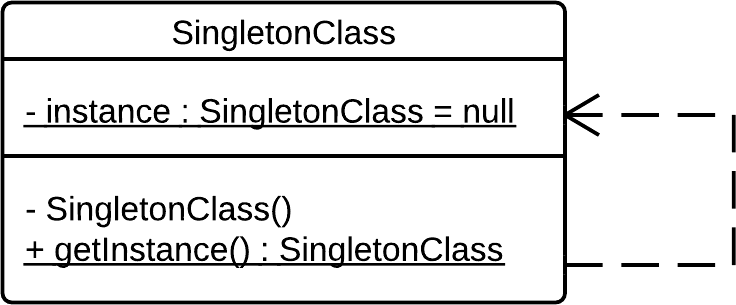
\includegraphics[width=.8\textwidth]{singleton}
\caption{Diagramma ad alto livello del pattern Singleton.}\label{fig:singleton}
\end{figure}
\subsubsection{Vantaggi derivanti}
\begin{itemize}
\item accesso controllato a un'unica istanza;
\item riduzione dello spazio dei nomi in quanto riduce l'uso di variabili globali;
\item permette di gestire un numero variabile di istanze.
\end{itemize}
\subsubsection{Componenti che lo implementano}
%\item ******************************************************

\subsection{State}
\subsubsection{Scopo}
Permette ad un oggetto di cambiare il suo comportamento al variare del suo stato interno, quindi a run-time. L'oggetto si comporterà come se avesse cambiato la sua classe.
\subsubsection{Diagramma esemplificativo}
\begin{figure}[h]
\centering

\includegraphics[width=.7\textwidth]{state}
\caption{Diagramma ad alto livello del pattern State.}\label{fig:state}
\end{figure}
\subsubsection{Vantaggi derivanti}
\begin{itemize}
\item specializza il comportamento associato ad uno stato;
\item rende esplicita la transazione si stato (tale condizione è espressa esplicitamente);
\item condivisione di oggetti di stato.
\end{itemize}
\subsubsection{Componenti che lo implementano}
\begin{itemize}
\item Gestione dello Stato
\end{itemize}
\clearpage

\section{Introduzione all'architettura di sistema}
\clearpage

\section{Architettura MyTalk-Server}
%TODO: da completare
Infine, si fa notare che i nomi di tutte le classi riportate nella sezione sono implicitamente parte del package \texttt{org.softwaresynthesis.server} pertanto tale prefisso sarà omesso nella loro denominazione.

\subsection{Componenti evidenziate}

\subsubsection{Gestione Database}
\begin{description}
\item{\scshape\bfseries Descrizione:}\\
Gestione Database è la componente che si occupa di rappresentare la struttura del database relazionale su cui poggia l'applicativo. Le singole classi in esso definite rappresentano quindi le tabelle del database. In termini tecnici Gestione Database implementa il design pattern DAO\@.

Tramite questa componente, il sistema potrà quindi effettuare operazione di lettura e scrittura di entità all'interno del database. Le classi che costituiscono la componente dovranno quindi essere dotate di:

\begin{itemize}
	\item metodi getter per restituire i singoli attributi dell'istanza;
	\item metodi setter per garantire un corretto inserimento dei dati prima di registrare l'istanza nel database.
\end{itemize}

Si informa inoltre che le classi di tale componente dovranno interagire con il \underline{framework} Hibernate, al fine di ottenere lo scopo precisato.

	\item{\scshape\bfseries Diagramma delle classi:}
	\item{\scshape\bfseries Classi utilizzate:}
\begin{itemize}
  \item \texttt{dao.AudioMessage}
  \item \texttt{dao.AudioVideoMessage}
  \item \texttt{dao.IAudioMessage}
  \item \texttt{dao.IAudioVideoMessage}
  \item \texttt{dao.IGroup}
  \item \texttt{dao.IUserData}
  \item \texttt{dao.StandardGroup}
  \item \texttt{dao.StandardUserData}
\end{itemize}
\end{description}

\begin{itemize}
	\item \texttt{connection.ISocket}
	\item \texttt{connection.WebSocketAdapter}
\end{itemize}

\subsubsection{Gestione connessione}
\begin{description}
	\item{\scshape\bfseries Descrizione:}\\
Tale componente ingloba le classi destinate a stabilire le routine di connessione. Il server ha la consapevolezza degli oggetti rappresentati una connessione tra client. Si ricorda infatti che: ``ogni cliente per comunicare con altri, deve prima connettersi al server e richiedere a questo un oggetto rappresentante la linea di comunicazione con il destinatario''. Le specifiche di tale oggetto sono descritte dall'interfaccia \texttt{connection.ISocket}.

Al fine di rendere l'architettura di tale componente il più manutenibile possibile, si è deciso di usare il pattern Adapter. In pratica esternamente il sistema ha esclusivamente la conoscenza dell'interfaccia \texttt{connection.ISocket}. Quindi l'esterno è svincolato dal conoscere il tipo preciso di protocollo di connessione (che ricordiamo nel nostro caso essere \texttt{da\_definire}). Poiché la classe che implementa il protocollo di comunicazione esiste già, nasce l'esigenza di ``adattare'' tale classe alla nostra interfaccia (\texttt{connection.ISocket}). Ciò giustifica l'esistenza della classe \texttt{connection.WebSocketAdapter}.
	\item{\scshape\bfseries Diagramma delle classi:}
	\item{\scshape\bfseries Classi utilizzate:}
\begin{itemize}
  \item \texttt{connection.ISocket}
  \item \texttt{connection.WebSocketAdapter}
  \item \texttt{da\_definire}
\end{itemize}
\end{description}

\subsubsection{Gestione rubrica}
\begin{description}
	\item{\scshape\bfseries Descrizione:}\\
La rubrica è organizzata in gruppi e sono previste due categorie di default: la \textit{blacklist} e la \textit{whitelist}. L'utente può aggiungere ulteriori gruppi in base alle sue esigenze ma esclusivamente all'interno della \textit{whitelist}. Per trattare in maniera omogenea i gruppi di contatti e i singoli contatti si è utilizzato il design pattern Composite.

In particolare, \texttt{abook.IContact} rappresenta l'interfaccia principale comune a ogni tipologia di contatto e viene estesa dalle due interfacce \texttt{dao.IUserData} e \texttt{dao.IGroup}. La componente comprende anche l'interfaccia \texttt{abook.IAddressBook} e la relativa implementazione \texttt{abook.AddressBook}. Nell'implementazione specificata \texttt{abook.Addressbook} vincola il sistema a garantire che ogni utente abbia i due gruppi di default sopra descritti, come richiesto dai requisiti.

	\item{\scshape\bfseries Diagramma delle classi:}
	\item{\scshape\bfseries Classi utilizzate:}\\
\begin{itemize}
  \item \texttt{abook.AddressBook}
  \item \texttt{abook.IAddressBook}
  \item \texttt{abook.IContact}
  \item \texttt{dao.IGroup}
  \item \texttt{dao.IUserData}
\end{itemize}

\end{description}

\subsubsection{Gestione stato}
\begin{description}
	\item{\scshape\bfseries Descrizione:}\\
	Le classi di tale componente sono utilizzate per gestire lo stato degli utenti, permettendo un comportamento diverso delle istanze di \texttt{dao.StandardUserData} a seconda dello stato in cui si trova l'utente corrispondente. Gli stati possibili sono ``online'' e ``offline'' che sono rappresentati dalle classi \texttt{state.StateOnline} e \texttt{state.StateOffline} rispettivamente.
	
	Gli utenti che si trovano nello stato online possono trovarsi in due situazioni: ``occupato'' o ``disponibile'', rappresentati a loro volta dalle classi \texttt{state.StateOccupied} e \texttt{state.StateAvailable}. L'utente si troverà nello stato ``occupato'' solo se è impegnato in una conversazione. Lo stato può essere controllato solo dal sistema in risposta agli eventi di connessione e di chiamata ma non è direttamente accessibile dall'utente.
	
	Ad esempio, la chiamata viene trattata in modo differente a seconda che l'utente si trovi nello stato ``disponibile'' o ``occupato''/``offline'', dal momento che nel primo caso la chiamata va a buon fine mentre nel secondo verrà attivato il meccanismo di segreteria telefonica.
	
	Inoltre, i cambiamenti di stato vengono notificati a tutti gli utenti presenti in rubrica tali che si trovano nello stato online.
	
	\item{\scshape\bfseries Diagramma delle classi:}
	\item{\scshape\bfseries Classi utilizzate:}\\ 
	\begin{itemize}
          \item \texttt{dao.StandardUserData}
          \item \texttt{state.IState}
          \item \texttt{state.StateAvailable}
          \item \texttt{state.StateOccupied}
          \item \texttt{state.StateOffline}
          \item \texttt{state.StateOnline}
	\end{itemize}
\end{description}

\subsubsection{Gestione segreteria}
\begin{description}
	\item{\scshape\bfseries Descrizione:}\\
Il sistema segreteria telefonica corrisponde all'interfaccia \texttt{message.IMessageBox} e alla relativa implementazione \texttt{message.StandardMessageBox} che permettono un accesso centralizzato all'insieme di messaggi che un determinato utente ha ricevuto.

I messaggi audio e audio/video sul server sono rappresentati dalle classi \texttt{dao.IAudioMessage} (implementata da \texttt{dao.AudioMessage}) e \texttt{dao.IAudioVideoMessage} (implementata da \texttt{dao.AudioVideoMessage}) rispettivamente. L'onere di caricare in memoria e gestire l'interno contenuto del messaggio è posticipato al momento di effettiva necessità mediante l'utilizzo dei \textit{virtual proxy} corrispondenti alle classi \texttt{message.AudioMessageProxy} e \texttt{message.AudioVideoMessageProxy}.
	\item{\scshape\bfseries Diagramma delle classi:}
	\item{\scshape\bfseries Classi utilizzate:}
\begin{itemize}
  \item \texttt{dao.AudioMessage}
  \item \texttt{dao.AudioVideoMessage}
  \item \texttt{dao.IAudioMessage}
  \item \texttt{dao.IAudioVideoMessage}
  \item \texttt{message.AudioMessageProxy}
  \item \texttt{message.AudioVideoMessageProxy}
\end{itemize}
\end{description}

\subsubsection{Façade del server}
\begin{description}
	\item{\scshape\bfseries Descrizione:}\\
L'interfaccia \texttt{IServerFacade} e la relativa implementazione \texttt{StandardServerFacade}, nella quale si è scelto di applicare il design pattern Singleton, forniscono una sorta di interfaccia alle funzionalità offerte dal sottosistema server alle componenti che risiedono nel client. Le funzionalità esposte consentono di gestire i messaggi presenti in segreteria, le richieste di comunicazione con altri utenti il login/registrazione degli utenti.
	\item{\scshape\bfseries Diagramma delle classi:}
	\item{\scshape\bfseries Classi utilizzate:}\\
\begin{itemize}
  \item \texttt{IServerFacade}
  \item \texttt{StandardServerFacade}
\end{itemize}
\end{description}

\subsection{Classi utilizzate}

%\subsubsection{Template classe X}
%\begin{description}
%	\item{\scshape\bfseries Descrizione:} 
%	\item{\scshape\bfseries Diagramma della classe:}
%	\item{\scshape\bfseries Componenti che ne fanno uso:} 
%\end{description}

\subsubsection{mytalk.server.dao.IAudioMessage}
\begin{description}
	\item{\scshape\bfseries Descrizione:} 
	\item{\scshape\bfseries Componenti che ne fanno uso:} 
\end{description}

\subsubsection{mytalk.server.dao.AudioMessage}
\begin{description}
	\item{\scshape\bfseries Descrizione:} 
	\item{\scshape\bfseries Componenti che ne fanno uso:} 
\end{description}

\subsubsection{mytalk.server.dao.IAudioVideoMessage}
\begin{description}
	\item{\scshape\bfseries Descrizione:} 
	\item{\scshape\bfseries Componenti che ne fanno uso:} 
\end{description}

\subsubsection{mytalk.server.dao.IGroup}
\begin{description}
	\item{\scshape\bfseries Descrizione:} 
	\item{\scshape\bfseries Componenti che ne fanno uso:} 
\end{description}

\subsubsection{mytalk.server.dao.StandardGroup}
\begin{description}
	\item{\scshape\bfseries Descrizione:} 
	\item{\scshape\bfseries Componenti che ne fanno uso:} 
\end{description}

\subsubsection{mytalk.server.dao.IUserData}
\begin{description}
	\item{\scshape\bfseries Descrizione:} 
	\item{\scshape\bfseries Componenti che ne fanno uso:} 
\end{description}

\subsubsection{mytalk.server.dao.StandardUserData}
\begin{description}
	\item{\scshape\bfseries Descrizione:} 
	\item{\scshape\bfseries Componenti che ne fanno uso:} 
\end{description}

\subsubsection{mytalk.server.connection.ISocket}
\begin{description}
	\item{\scshape\bfseries Descrizione:} 
	\item{\scshape\bfseries Componenti che ne fanno uso:} 
\end{description}

\subsubsection{mytalk.server.connection.WebSocketAdapter}
\begin{description}
	\item{\scshape\bfseries Descrizione:} 
	\item{\scshape\bfseries Componenti che ne fanno uso:} 
\end{description}

\subsubsection{mytalk.server.abook.IContact}
\begin{description}
	\item{\scshape\bfseries Descrizione:} 
	\item{\scshape\bfseries Componenti che ne fanno uso:} 
\end{description}

\subsubsection{mytalk.server.abook.IAddressBook}
\begin{description}
	\item{\scshape\bfseries Descrizione:} 
	\item{\scshape\bfseries Componenti che ne fanno uso:} 
\end{description}

\subsubsection{mytalk.server.abook.AddressBook}
\begin{description}
	\item{\scshape\bfseries Descrizione:} 
	\item{\scshape\bfseries Componenti che ne fanno uso:} 
\end{description}

\subsubsection{mytalk.server.state.IState}
\begin{description}
	\item{\scshape\bfseries Descrizione:} 
	\item{\scshape\bfseries Componenti che ne fanno uso:} 
\end{description}

\subsubsection{mytalk.server.state.StateOnline}
\begin{description}
	\item{\scshape\bfseries Descrizione:} 
	\item{\scshape\bfseries Componenti che ne fanno uso:} 
\end{description}

\subsubsection{mytalk.server.state.StateOffline}
\begin{description}
	\item{\scshape\bfseries Descrizione:} 
	\item{\scshape\bfseries Componenti che ne fanno uso:} 
\end{description}

\subsubsection{mytalk.server.state.StateAvailable}
\begin{description}
	\item{\scshape\bfseries Descrizione:} 
	\item{\scshape\bfseries Componenti che ne fanno uso:} 
\end{description}

\subsubsection{mytalk.server.state.StateOccupied}
\begin{description}
	\item{\scshape\bfseries Descrizione:} 
	\item{\scshape\bfseries Componenti che ne fanno uso:} 
\end{description}

\subsubsection{mytalk.server.message.IMessageBox}
\begin{description}
	\item{\scshape\bfseries Descrizione:} 
	\item{\scshape\bfseries Componenti che ne fanno uso:} 
\end{description}

\subsubsection{mytalk.server.message.StandardMessageBox}
\begin{description}
	\item{\scshape\bfseries Descrizione:} 
	\item{\scshape\bfseries Componenti che ne fanno uso:} 
\end{description}

\subsubsection{mytalk.server.message.AudioMessageProxy}
\begin{description}
	\item{\scshape\bfseries Descrizione:} 
	\item{\scshape\bfseries Componenti che ne fanno uso:} 
\end{description}

\subsubsection{mytalk.server.message.AudioVideoMessageProxy}
\begin{description}
	\item{\scshape\bfseries Descrizione:} 
	\item{\scshape\bfseries Componenti che ne fanno uso:} 
\end{description}

\subsubsection{mytalk.server.IServerFacade}
\begin{description}
	\item{\scshape\bfseries Descrizione:} 
	\item{\scshape\bfseries Componenti che ne fanno uso:} 
\end{description}

\subsubsection{mytalk.server.StandardServerFacade}
\begin{description}
	\item{\scshape\bfseries Descrizione:} 
	\item{\scshape\bfseries Componenti che ne fanno uso:} 
\end{description}

\subsection{Diagramma del package}

\subsection{Diagramma delle classi}
\clearpage

\section{Architettura MyTalk-client Universale}

\subsection{Componenti evidenziate}

\subsubsection{Gestione rubrica}
\begin{description}
	\item{\scshape\bfseries Descrizione:} 
	\item{\scshape\bfseries Diagramma delle classi:}
	\item{\scshape\bfseries Classi utilizzate:} 
\end{description}

\subsubsection{Gestione comunicazione}
\begin{description}
	\item{\scshape\bfseries Descrizione:} 
	\item{\scshape\bfseries Diagramma delle classi:}
	\item{\scshape\bfseries Classi utilizzate:} 
\end{description}

\subsection{Classi utilizzate}

\subsubsection{mytalk.client.Contact}
\begin{description}
	\item{\scshape\bfseries Descrizione:} 
	\item{\scshape\bfseries Componenti che ne fanno uso:} 
\end{description}

\subsubsection{mytalk.client.IClient}
\begin{description}
	\item{\scshape\bfseries Descrizione:} 
	\item{\scshape\bfseries Componenti che ne fanno uso:} 
\end{description}

\subsubsection{mytalk.client.StandardClient}
\begin{description}
	\item{\scshape\bfseries Descrizione:} 
	\item{\scshape\bfseries Componenti che ne fanno uso:} 
\end{description}

\subsubsection{mytalk.client.IPresenterFacade}
\begin{description}
	\item{\scshape\bfseries Descrizione:} 
	\item{\scshape\bfseries Componenti che ne fanno uso:} 
\end{description}

\subsubsection{mytalk.client.StandardServerFacade}
\begin{description}
	\item{\scshape\bfseries Descrizione:} 
	\item{\scshape\bfseries Componenti che ne fanno uso:} 
\end{description}

\subsection{Diagramma del package}

\subsection{Diagramma delle classi}
\clearpage

\section{Architettura MyTalk-clientSoftwareSynthesis}

\subsection{Componenti evidenziate}

\subsubsection{Template della componente X}
\begin{description}
	\item{\scshape\bfseries Descrizione:} 
	\item{\scshape\bfseries Diagramma del package:}
	\item{\scshape\bfseries Classi utilizzate:} 
\end{description}

\subsection{Classi utilizzate}

\subsubsection{Template classe X}
\begin{description}
	\item{\scshape\bfseries Descrizione:} 
	\item{\scshape\bfseries Diagramma della classe:}
	\item{\scshape\bfseries Componenti che ne fanno uso:} 
\end{description}

\subsection{Diagramma del package}

\subsection{Diagramma delle classi}
\clearpage

\section{Conclusioni sull'architettura}

\subsection{Diagrammi delle attività}

\subsection{Diagrammi di sequenza}
\clearpage

\section{Tracciamenti}
Nella seguente sezione vengono proposti tutti i tracciamenti eseguiti mediante il sistema Synthsis Requirment Manager. I tracciamenti proposti sono giustificati dalle seguenti due motivazioni:

\begin{itemize}
	\item Dimostrare il soddisfacimento per necessarietà e sufficienza della corrispondenza tra gli elementi tracciati (e.g. una componente deve rispondere necessariamente alle esigenze di uno o più requisiti, tali insomma che ne giustifichino l'esistenza. D'altro canto è richiesto che ogni requisito definito in fase d'analisi sia soddisfatto e risolto da almeno una componente).
	\item dare una lettura generale delle varie: componenti, requisiti, design pattern e classi.
\end{itemize}

\subsection{Tracciamenti Requisiti-Componenti}

\subsection{Tracciamenti Componenti-Requisiti}

\subsection{Tracciamenti Componenti-DesignPattern}

\subsection{Tracciamenti DesignPattern-Componenti}

\subsection{Tracciamenti Componenti-Classi}

\subsection{Tracciamenti Classi-Componenti}

\end{document}